%!TEX root = main.tex
%%%%%%%%%%%%%%%%%%%%%%%%%%%%%%%%%%%%%%%%%%%%%%%%%%%%%%%%%%%%%%%%%%%%%%%%%%%%%%%%%%%%%%%%%%%%%%%%%%%%%%
%
%   Filename    : chapter_2.tex 
%
%   Description : This file will contain your Review of Related Literature.
%                 
%%%%%%%%%%%%%%%%%%%%%%%%%%%%%%%%%%%%%%%%%%%%%%%%%%%%%%%%%%%%%%%%%%%%%%%%%%%%%%%%%%%%%%%%%%%%%%%%%%%%%%

\chapter{Review of Related Literature}
\label{sec:relatedlit}
\begin{comment}
then for team MusicG my suggested columns would be 
2.1 Authors | Focus (if melody, chord, progression, sequence) | Model (what math formula or name did they use no need to put formula sa table) 
2.2 Authors | Name of Tool | Platform | Input Type | Algorithm (what they used to generate sequences)
2.3 Authors | Name of Tool | How many testers | Comments  and other  reported findings
\end{comment}

This chapter discusses the features, capabilities, and limitations of existing research, algorithms, or software that are related/similar to the study.

\section{Mathematical Analysis of Music and its Melodies}
This section provides an analysis on different works towards modeling music and melody mathematically. Because of the musical nature of this study, it is important to understand the terms used in music and how past studies have made steps to mathematically represent music and its elements.

\citet{loy2011musimathics} defines music as a creative form of art whose medium is sound. It includes several elements (e.g., note, pitch, rhythm, etc.) which can be represented mathematically. One such element is melody. The melody plays an important part in music \citep{unehara2001composition,unehara2005music} as it is the sequence of notes that define the sound of music \citep{ryynanen2008automatic}. 

The melody will most likely make the most impact on the listener \citep{jarret2008music}. These succession of notes usually define the body or general idea of a composition through the form it takes in a musical framework \citep{jarret2008music}. Whether this form contains quick tempos that provoke the listener into motion or a slow tempo leaving the listener relaxed, it is important for a composer to add melodies that can bring the composition to life \citep{jarret2008music}. 

% The listener will more than likely be impacted the most by the melody of the composition \citep{jarret2008music}. These succession of notes usually define the body or general idea of a composition through the form it takes in a musical framework \citep{jarret2008music}. Whether this form contains quick tempos that provoke the listener into motion or a slow tempo leaving the listener relaxed, it is important for a composer to add melodies that can bring the composition to life \citep{jarret2008music}. 

\citet{poliner2007melody} provided a more musicological definition of melody, which is the single pitch sequence that a listener would recognize to be the ``essence'' or the ``soul'' of the composition being listened to. This definition was later supported in the study of \citet{salamon2012melody}, where they attempted to extract the melody from music signals by identifying the most significant pitch in a composition. 

Both \citet{poliner2007melody} and \citet{salamon2012melody} borrowed the mathematical representation of melody that was provided by \citet{goto2004real} in his earlier study. \citeauthor{goto2004real} represented melody through a predominant-F0 estimation method, or what he called \textit{PreFEst}, where F0 denotes the fundamental frequency. In this method, the melody is identified by finding the strongest, or most dominant harmonic structure within specific regions of the audio signal. 

\begin{comment}
However, according to \citet{dannenberg1993music}, representing music mathematically is difficult as there are some elements involved that cannot be represented by math, like the emotion involved when playing music. Despite this, research has gone into analyzing the elements of music that can be represented mathematically, such as pitch, which has a key role in music as it determines how ``high'' or ``low'' a note would sound.
\end{comment}

On the other hand, \citet{dorfler2001time} links music signals to Gabor analysis, a method of analyzing music by separating it into segments referred to as frames \citep{gabor1946theory}. Given that music has many high-level and low-level music features that can be represented in the mathematical aspect, \citet{dorfler2001time} relates how music is very similar to a Hilbert Space in terms of digital signal processing. This can be modeled into a set of energy signals that contains many features that she considers to belong in a space of square-integrable functions \begin{math} {L}^2 (\mathbb{R}),\mathbb{R} \rightarrow  \mathbb{C}  \end{math}. Following this, \citet{dorfler2001time} mentions that such spaces which are capable of containing complex set of features are usually infinite in form. However, she mentions that though music may contain such set of features, it is not infinite but rather it is continuous in form. To accommodate this, she proposed a modification of the existing model that accommodates the limitations in finiteness.

\begin{comment}
\begin{equation}
\label{eq:1}
l^2(\mathbb{Z}):=\left\{f:\mathbb{Z}\rightarrow\mathbb{C}\sum_{n=-\infty}^\infty|f(n)|^2<\infty \right\}
\end{equation}

\begin{equation}
\label{eq:2}
(f*g)(n)=\sum_m f(m)g(n-m)
\end{equation}
\end{comment}

She introduces that music is usually measured in length \begin{math}L\end{math} as members of the complex vector space \begin{math}\mathbb{C}^L\end{math} where finite sequences are treated as period sequences in forms of what she introduces as \textit{circular extensions} of the said signals coming from \begin{math}\mathbb{Z}_L = \mathbb{Z} mod L\end{math} \citep{dorfler2001time}. 

This was supported by the earlier work of \citet{fucks1962mathematical} where he focused on analyzing the statistical aspects of music, specifically the frequency distribution of the pitch in music present from 1500 - 1960. This time, he represented the such sequences in what he calls \textit{kurtosis} (\textit{K}), that is defined as the measure of the sharpness of the peak in frequency distributions. In retrospect, the length of digital signals introduced by \cite{dorfler2001time} are similar in meaning to the frequencies measured by \cite{fucks1962mathematical}. 

\begin{comment}
\begin{equation}
\label{eq:3}
K = \frac{\mu^4}{\sigma^4}
\end{equation}

\begin{equation}
\label{eq:4}
\mu_v = \sum_x(x-\overline{x})^v\cdot p_x
\end{equation}

\begin{equation}
\label{eq:5}
\overline{x} = \sum_x\cdot p_x
\end{equation}
\end{comment}

\citet{voss1978noise} initiated the study on the spectral density of music, where spectral density is defined as a function that determines the strength of the energy of a signal \citep{stoica1997introduction, martin2001noise}. In their study, \citeauthor{voss1978noise} found that music that exhibited a spectral density of $\frac{1}{f}$ noise, where \textit{f} is the frequency, was particularly pleasing to hear. This was mainly due to how the certain frequency was similar to that of human communication. The other spectral density that was observed, $\frac{1}{f^2}$ noise, was considered less pleasant \citep{gunduz2005mathematical}, and too correlated \citep{voss1978noise,nettheim1992on}. 

\citet{buxton1978the} investigated the possibility of modeling music as data structures in what he calls \textit{hierarchies}. \citeauthor{buxton1978the} defined a \textit{hierarchy} as a structure that contains either a single note, or another \textit{hierarchy}. He observed that a musical composition can be separated into chunks and be played separately. Within these said chunks could be other smaller chunks or up to just a single note. By treating music as \textit{hierarchies} or chunks, the music could have multiple levels where whenever a level is played, all the levels beneath it would also be played. The composer would have the ability to choose smaller chunks or lower levels of the music to be able to play a certain part. This system of representing music as \textit{hierarchies} was also supported by \citet{brinkman1984data} in his study with the use of linked lists. 

The same ideology was also present in the later study of \citet{bozhanov2014computoser}. In this study, music was modeled as a set of rules. A composition is considered as a structure, with its own properties like rhythm, meter, scale, etc. Similarly, the study of \citep{schulze2011music} also represented music using rules, but more specifically, Markov chains. The composition is modeled using probabilistic automata with the states as its notes.

Shown in Table \ref{tab:rsotmaomaim} is a summary of the reviewed works and a comparison of their focus and model.

\begin{landscape} % Landscape page
\begin{table} [!htbp]  

        \captionof{table}{Related Studies on the Mathematical Analysis of Music and its Melodies} \label{tab:rsotmaomaim} 
   \vspace{0.20cm}    
        \begin{tabular}{|p{5cm}|p{5cm}|p{5cm}|p{5cm}|} %{|l|l|l}
        \hline 

       Authors & Focus & Theory/Principle & Contributions/Details \\ \hline
       
       \citet{goto2004real, salamon2012melody, poliner2007melody} & Melody & Fundamental Frequency (F0) & Melody is the most dominant harmonic structure \\ \hline
       
       \citet{dorfler2001time} & Music as a digital signal & Gabor analysis \& Hilbert space & Music contains features that are infinite in form, but it is still continuous \\ \hline
       
       \citet{fucks1962mathematical} & Pitch & Kurtosis and Frequency Distribution & The pitch can be analyzed in terms of peaks in frequency distributions \\ \hline
       
       \citet{voss1978noise, nettheim1992on, gunduz2005mathematical} & Frequency, Pitch \& Melody & Spectral Density & Music generally exhibits a spectral density of $\frac{1}{f}$ noise \\ \hline
       
       \citet{buxton1978the, brinkman1984data} & Music & Hierarchies or Chunks & A composition is a structure that can be separated into substructures \\ \hline
       
       \citet{bozhanov2014computoser} & Music & Rule-based algorithm & A composition can be modeled using a structure with rules and properties \\ \hline
       
       \citet{schulze2011music} & Music & Markov chains and Probabilistic automata & A composition can be represented as a set of states \\ \hline
       
        \end{tabular}
\end{table}
\end{landscape}


\section{Musical Composition \& Recommendation Systems}
This section contains a review of research papers that discuss systems that produced musical compositions with the aid of various algorithms.

Musical composition systems that attempted to augment the composition process have already been developed in the past. \citet{eigenfeldt2010realtime} generated music through their system that makes use of Markov models, a method of generating sequences or melodies by deriving features from a provided corpus. However, this also resulted in an inability to generate a deeper, or a varied structure of music, which was also expressed in the earlier study of \citet{ames1989markov}. 

% The advantage of Markov models were that they did not need to follow any rules. 

\citet{herremans2016morpheus} developed MorpheuS which is a system that generates music with the use of tension profiles that are computed from a template of a musical piece. The system uses an optimization approach which avoids the recursive behavior of Markov models during pattern finding to avoid the use of non-standard hierarchical models which lack efficiency \citep{herremans2016morpheus}. 

\begin{comment}
There are other approaches which yield more efficient results \citep{damlen1999gibbs}. COSIATEC and SIATECCompress are two greedy compression algorithms used by MorpheuS that find patterns in a given template piece.
\end{comment}

% Another similar system is SuperWillow which was developed in the study of \citet{schulze2011music}. It uses symbolic music as the representation of partially composed music. They conducted a partial Turing test wherein respondents were asked to identify which of the two given musical compositions was composed by a human being. 38\% of the respondents incorrectly identified the computer-generated musical composition as a human composition. The SuperWillow uses LearnPSA algorithm which generates prediction suffix trees that is converted to PSA. Probably approximately correct learning model (PAC) prompted the PSA algorithm. After composition analysis, the objects generated are then used in order to compose or imitate music using the training data. Distribution sampling is used in order to generate music instead of calculating the probable sequence of notes.

% Another similar system is SuperWillow which was developed in the study of \citet{schulze2011music}. It uses symbolic music as the representation of partially composed music. The SuperWillow uses LearnPSA algorithm which generates prediction suffix trees that is converted to PSA. Probably approximately correct learning model (PAC) prompted the PSA algorithm. After composition analysis, the objects generated are then used in order to compose or imitate music using the training data. Distribution sampling is used in order to generate music instead of calculating the probable sequence of notes.

Another similar system is SuperWillow which was developed in the study of \citet{schulze2011music}. SuperWillow takes in musical data in the form of MusicXML. The data is then used to generate Markov chains and probabilistic automatons to model musical elements. After composition analysis, the objects generated are then used in order to compose or imitate music similar to the training data. Distribution sampling is used in order to generate music instead of calculating the probable sequence of notes.

\citet{kikuchi2014automatic} approached musical metacreation using a genetic algorithm to generate melody. The approach used N-gram models to represent rhythm and pitch in each melody block to use in the algorithm. In order to produce melodies, musical features are likened to human genes, which contain different properties. The first part of the process involves random generation of initial individuals that are based on rhythm, pitch, and chord progression. Fitness calculation will then be done to determine which individuals have similar musical features for the crossover. The parent individuals will be used to generate new individuals, repeatedly.

% A genetic algorithm was also used the Composition in Genetic Approach (CONGA) \citep{tokui2000music}. The system takes in a fitness score or evaluation in order to generate a better rhythm. It suggests that people have various preferences based on their personal fitness scores, which can be subjective. It uses both the genetic algorithm and genetic programming which complements each other in creating structured rhythm. Every time the user submits a fitness evaluation, the genetic algorithm and genetic programming starts to improve or sustain the rhythm produced based from their input and returns a rhythm which is needed to be evaluated by the user again.

A genetic algorithm was also used the Composition in Genetic Approach (CONGA) \citep{tokui2000music}. The system takes in a fitness score or evaluation in order to generate a better rhythm. Every time the user submits a fitness evaluation, the genetic algorithm and genetic programming starts to improve or sustain the rhythm produced based from their input and returns a rhythm which is needed to be evaluated by the user again.

The study of \cite{geis2008creating} developed a system that used Ant Colony Optimization (ACO) for the generation. ACO also depended on multiple iterations of training similar to previous studies that used genetic algorithms \citep{tokui2000music,kikuchi2016music}. It was believed that composers sometimes broke musical rules in their compositions. This study attempted to model that behavior with how ants followed certain pheromones while searching for food, hence the ACO algorithm. However, the study's limitation was that it did not include a Graphical User Interface (GUI) to allow for real time input \citep{geis2008creating}.

% The study of \cite{geis2008creating} developed a system that used Ant Colony Optimization (ACO) for the generation. ACO also depended on multiple iterations of training similar to previous studies that used genetic algorithms \citep{tokui2000music,kikuchi2016music}. It was remarked in the study that there were great composers that broke musical rules, and they wanted to mimic those sudden changes through the ACO algorithm which mimicked how ants followed certain pheromones while searching for food \citep{geis2008creating}. Despite the music generated from the system being satisfactory to the musical criteria presented by the researchers, a suiting Graphical User Interface (GUI) was not developed for real time input \citep{geis2008creating}.

Aforementioned systems focused on musical metacreation, leaving aside user experience, resulting in a lack of interaction. Hyperscore, developed by \citet{farbood2004hyperscore}, focused on user experience by designing an appropriate graphical user interface for the musical structure. The idea behind Hyperscore was to allow people to compose short melodies with minimal expertise in musical composition.  \citeauthor{farbood2004hyperscore} believed that the new method of interaction allowed users to have an expressive way of shaping musical direction.

\citet{kikuchi2016music} supported the idea of musical composition with interaction. They developed a music composition tool that used the Microsoft Surface Pro 3 and the Surface Pen, which enabled the use of gestures for its interactions. It provides users possible pitches to continue writing the composition that is being written. The system involves extraction of pitch transition and rhythm from a musical piece provided by the user as input. Those features are used to generate the recommended pitches and present them to the user in real time. They are then stored in a local SQLite database and searched every time the system is trying to find the right pitch or pitches to recommend to display.

Another system that included a user interface was Computoser, developed by \citet{bozhanov2014computoser}. Similar to previous studies, it uses a rule-based approach but includes probabilistic characteristics in the algorithm for generating music. The rules in the system were based on music theory and with the help of some experts \citep{bozhanov2014computoser}. As seen in Figure \ref{fig:computoser-preference}, the system enables the user to adjust the weights in the preferences with which the music is generated. The result is a composition based to the choices the user made and can be immediately played in the web browser through a media player present in the website as seen in Figure \ref{fig:computoser-media}. 

\begin{figure}[H]
	\centering
	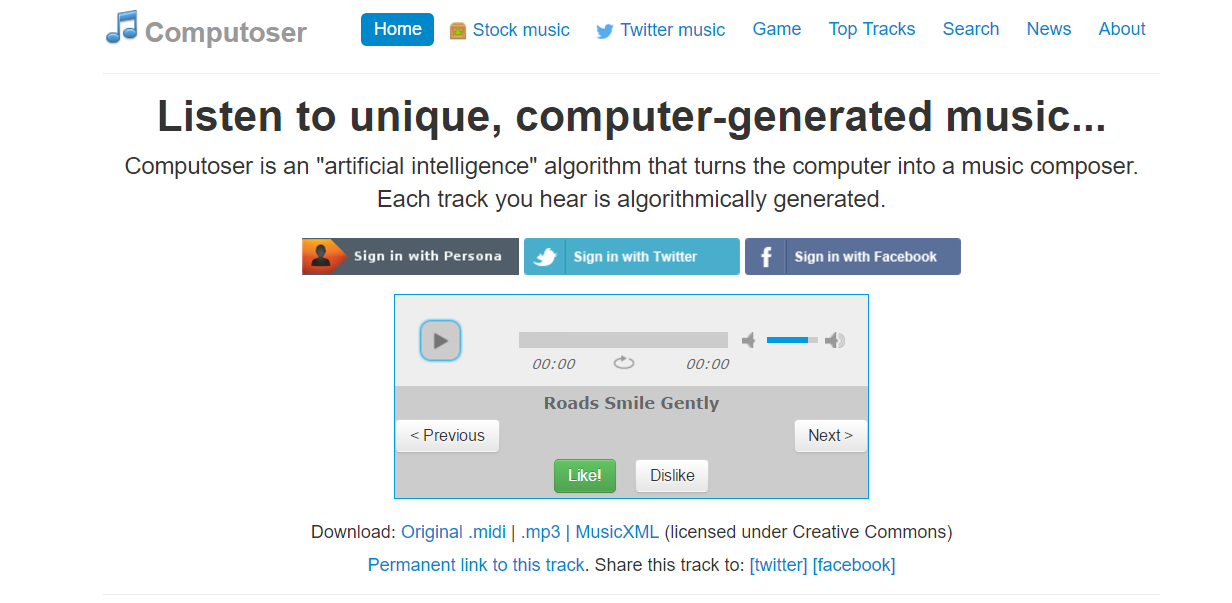
\includegraphics[scale=0.5]{ComputoserMediaPlayer}
    \caption{\textit{Computoser} media player \citep{bozhanov2014computoser}.}
    \label{fig:computoser-media}
\end{figure}

\begin{comment}
Another way to improve upon the process of musical composition is through focusing on what feels natural to the target users. Composers and musicians also feel with their body when composing music through instruments \citep{de2012playing}. In recent years, the use of touch interfaces have proven to feel more natural than using external input devices like the mouse \citep{travis2014comparative}. The use of gesture interactions through modern innovations like the touch screen is both an intuitive and interaction focused approach for a system \citep{epps2006a}. It is also mentioned in the study of \cite{travis2014comparative} that despite the general acceptance of the public with the innovation of touch, there are still facets of the technology that can be improved upon for the overall performance and usability of the touch screen \citep{travis2014comparative}.
\end{comment}

% FORMAT FOR A NEW ROW IN 2.2 : \citet{} & 1 & 2 & 3 & 4 \\ \hline

\begin{landscape} % Landscape page
\begin{table} [!htbp]  
\label{tab:rsomcrtas}        
        \captionof{table}{Related Studies on Musical Composition \& Recommendation Tools and Systems}
   \vspace{0.20cm}    
        \begin{tabular}{|p{3cm}|p{4cm}|p{3cm}| p{5cm} | p{5cm}| } %{|l|l|l}
        \hline 
       Authors & Name of Tool & Platform & Input/Modality & Algorithm \\ \hline
       
       \citet{ames1989markov,eigenfeldt2010realtime} & NA & NA & MIDI files & Markov models \\ \hline
      
       \citet{herremans2016morpheus} & MorpheuS & NA & Template piece & Tension profiles \\ \hline
       
       \citet{camurri1991harp} & HARP & NA & Source composition/piece & Networks\\ \hline
       
       \citet{tokui2000music, kikuchi2014automatic} & CONGA; NA & PC; NA & Fitness Score; NA & Genetic Algorithm with Genetic Programming; Genetic Algorithm with N-grams\\
        \hline
        
        \citet{kikuchi2016music} & Music Composition with Recommendation & Tablet (Microsoft Surface Pro 3) & Touch with the use of Surface Pen & Database of Features \\ \hline
        
        \citet{bozhanov2014computoser} & Computoser & Web & Form-Based & Hybrid Rule-Based, Probability Driven Algorithm \\
        \hline
        
        \citet{geis2008creating} & NA & PC & Length of melody \& Set of allowed pitches & Ant Colony Optimization \\
        \hline
      
        \end{tabular}
\end{table}
\end{landscape}

\section{Music Generation and Evaluation}

% In the current metrics of computer generated music evaluation, the objective is to make the music feel “expressive” wherein the sound of the music does not sound monotonous and complies with the unique changes every composer adds to their piece \citep{de2002ai}. It is where the music generated feels human, where it has these subtle differences in tempo, pitch, timbre, and volume \citep{bresin2000emotional}. Studies have found that monotony makes for a piece that will leave the human brain's neuron's fire rate decrease because of habituation \citep{baars1993cognitive} therefore creating a dull musical experience. The excitement of change can increase the rate of how a brain’s neurons fire leaving the mind filled with activity \citep{de2012playing}.

In the current metrics of computer generated music evaluation, the objective is to make the music feel “expressive” wherein the sound of the music does not sound monotonous and complies with the unique changes every composer adds to their piece \citep{de2002ai}. It is where the music generated feels human, and has these subtle differences in tempo, pitch, timbre, and volume \citep{bresin2000emotional}. Expressiveness is a criterion for music and is defined as how close a computer-generated melody is to its human counterpart \citep{de2002ai}. Evaluation metrics range from how a generated piece not only conforms to the musical metrics and standards, but also to the change in dynamics that are found within songs composed to evoke certain emotions within the audience by the artist \citep{bresin2000emotional}. 

% Expressiveness is a criterion for music and is defined as how close a computer-generated melody is to its human counterpart \citep{de2002ai}. Evaluation metrics range from how a generated piece not only conforms to the musical metrics and standards, but also to the change in dynamics that are found within songs composed to evoke certain emotions within the audience by the artist \citep{bresin2000emotional}. In the field of computing, these systems that generated music purely using the context of the data input or through some extra input by the user were referred to as computer systems for expressive music performance (CSEMP) \citep{miranda2010artificial}. 

The TempoExpress system aimed to produce expressive music from monotonous music recordings \citep{grachten2006a}. The system used a principle called case-based reasoning (CBR), where it used cases as knowledge for the computer to refer to when generating a musical piece. CBR was used because of how the nature of music can differ with every piece. It can contain all the specific changes in each musical piece \citep{de2012playing}. The evaluation was done through a survey of 92 participants and then run through a performance measure \citep{grachten2006a}.

Saxex, a system that generates expressive saxophone jazz solos, also uses CBR. CBR performed well to help the system deal with the dynamics, rubato, vibrato, articulation, and attack of the notes in the jazz solo generated by the system \citep{arcos1998saxex}. The resulting melodies where then run through a spectral modeling synthesis (SMS) technique then analyzed whether the music was expressive or not \citep{arcos1998saxex}.

An Imitative Multi-Agent Perform (IMAP) was used in the study of \citet{miranda2010artificial}. The IMAP mimics how people listen to music and use it as inspiration for their own composition. The system used rules to evaluate given music, and only used the highest rated music as inspiration. It was then tested using certain algorithms to evaluate its success when generating melodies after training \citep{miranda2010artificial}.

% There are also systems wherein evaluation was not strictly done after a melody was generated. An Imitative Multi-Agent Performer (IMAP) runs through the cycle of evaluating one another then composing their own music after reflecting on the music previously listened to that had a high rating \citep{miranda2010artificial}. This system mimics how people listen to music and use it as their inspiration for future work. The evaluation of an agent within the system is determined with a set of rules for easier control over the parameters in rating different kinds of expressive music \citep{miranda2010artificial}. IMAP was then tested for certain categories and run through algorithms to evaluate its success in generating melodies after training \citep{miranda2010artificial}. 

% There is a similarity between IMAP system and the study of \citet{dahlstedt2006musical}. Both used multiple agents for musical metacreation. The main difference between the two is \citeauthor{miranda2010artificial} used the agents for evaluation, while \citeauthor{dahlstedt2006musical} used the agents for the actual metacreation. However, the study's research objectives were not met due to the agents' immaturity \citep{dahlstedt2006musical}.

% There is a similarity between IMAP system and the study of \citet{dahlstedt2006musical} where multiple agents where used to do certain tasks in generating a system. These multi-agents differ in the individual tasks each agent performs where in the IMAP system of \citet{miranda2010artificial}, each agent evaluated and performed within the community of agents while the agents in \citet{dahlstedt2006musical}'s system were splitting the tasks in the process of music creation. It was remarked how the discipline of agents was still in its developing stage since their system was not able to achieve the research objectives at that time \citep{dahlstedt2006musical}.

% MorpheuS, developed in the study of \citet{herremans2016morpheus} makes use of an efficient search algorithm called variable neighborhood search which generates polyphonic music with themes and tension profiles. Making use of tension profiles are useful in the context of game of film music. The results of the system turns out to be favorable since it has been used in different events around the world. Although the results turn out to be favorable, the researchers plan to further improve the overall efficiency of the system. Other improvements in the system include the quality of musical output by imposing more restrictions regarding the playability and the analytical properties of a style of music.

MorpheuS, developed in the study of \citet{herremans2016morpheus}, was tested by playing the results of the system in different musical events around the world. Although the results turned out to be favorable, the researchers plan to further improve the overall efficiency of the system. Other improvements in the system include the quality of musical output by imposing more restrictions regarding the playability and the analytical properties of a style of music.

In the study of \citet{schulze2011music}, SuperWillow was evaluated through a partial Turing test. Respondents were asked to identify human compositions versus computer-generated compositions. It was found that 72\% of the respondents either could not tell the difference between the composition composed by the computer and the human, or preferred computer-generated compositions over human compositions.

\citet{kikuchi2016music} performed testing on users with little experience in musical composition. They compared their system with another composition tool that was a Piano-roll type. It was found that their system allowed for more variety in compositions compared to the other system. Despite this, the system was still limited to the pitch transitions and rhythm of the training input provided \citep{kikuchi2016music}.

% \citet{kikuchi2016music} tested the system they developed by letting a user that has limited experience in composing music use their software and a composition system which was Piano-roll type. Compared with the Piano-roll system, their system produced musical compositions with more variety. However, their system is limited to the pitch transitions and rhythm of the provided musical piece. The originality of the musical composition can be an issue when it comes to generated music \citep{farbood2001hyperscore}.

% In the system of \cite{geis2008creating}, an ACO algorithm was used to generate music. The algorithm was similar used natural occurrences similar to that of genetic evolution. It was evaluated through rules in every stage of developing the composition. In its melody creation stage, smoothness, contour, tendency tone resolution, tone color, and pitch of the final note in the melody was evaluated \citep{geis2008creating}. In the baroque harmonization stage, chord arrangement, voice distance, voice leading, harmonic progression, smoothness, and chord resolutions were factors in the final piece \citep{geis2008creating}. These rules were enforced along with weights and parameters that the ACO algorithm follows.

\citet{yiiksel2011automatic} also developed a software that utilized a genetic algorithm. Their system generated notes using a genetic algorithm with recurrent neural networks. The algorithm used properties such as note, octave, and duration. Although it was only tested by the researchers, it was found that the metacreated music was only viable after a number of evolutions have been made. 

% Another software that revolves around the genetic algorithm was developed by \citet{yiiksel2011automatic}. They developed a system where the notes are generated through a genetic algorithm alongside with recurrent neural networks hence, removing the need of interaction. The properties of each gene used in the genetic algorithm are the note, octave, and duration. Music produced from their software is seen viable only after a number of evolutions or generations have been made.

Alternatively, in the study of \citet{birchfield2003generative}, a genetic algorithm was used with consideration for musical emotion, meaning, and form. The testing found that average listeners found the metacreated music to be interesting. On the other hand, a focused intensity was noticed by the experts due to the shifting rhythms, gestures, and phrasing \citep{birchfield2003generative}. Although experts also noted that the music contained some idle sections. This affected the emotion evoked by the music \citep{birchfield2003generative}.

% A generative model with the consideration of musical emotion, meaning, and form was also developed with the genetic algorithm. \citet{birchfield2003generative} created this generative model that revolved around various rules in composing music which includes the theory by Leonard Meyer which focuses on structuring music to be effective in portraying emotion. The results from the average and expert listeners did not vary much from each other. Average listeners found the music produced by the algorithm to be interesting and assessed it to be having a local variation. On the other hand, a focused intensity was noticed by the experts which was due to the shifting rhythms, gestures, and phrasing \cite{birchfield2003generative}. Some idle sections were also noticed by the experts which could result in destroying the momentum of emotion being portrayed by the music.

%\newpage
%\afterpage{\clearpage}

\begin{landscape} % Landscape page
\begin{table} [!htbp]  
\label{tab:rsomgae}        
        \captionof{table}{Related Studies on Music Generation and Evaluation}
   \vspace{0.20cm}    
        \begin{tabular}{|p{3cm}|p{4cm}|p{4cm}| p{10.5cm} | } %{|l|l|l}
        \hline 
       Authors & Name of Tool & Testers & Comments and other findings \\ \hline
       \citet{kikuchi2016music} & Music Composition with Recommendation & 1 inexperienced composer & The compositions produced were found to have more variety compared to the other tested system. \\ \hline
       
       \citet{herremans2016morpheus} & MorpheuS & Played in concerts & The system can generate polyphonic music with themes and tension profiles. The output of this system was said to be promising and further improvements in terms of efficiency of this system could be done. \\ \hline
       
       \citet{schulze2011music} & SuperWillow & 256 Stellenbosch University professors and students & Found that 38\% of the respondents incorrectly identified the computer-generated composition as a human composition.  \\ \hline
       
        \citet{grachten2006a} & TempoExpress & 92 testers& The system used Case-Based Reasoning and was compared to Uniform Time Stretch and was found to be better for generating a tempo that was slower than the source tempo. \\ \hline
        
        \citet{arcos1998saxex} & Saxex & Only tested by the researchers & The results satisfied the criteria of expressiveness for dynamics, rubato, and vibrato but it still needed work for the articulation and attack. \\ \hline 
        
        \citet{yiiksel2011automatic} & N/A & Only tested by the researchers & Generated music that has passed through many generations can be judged as acceptable. \\ \hline
        
        \citet{birchfield2003generative} & N/A & Tested on average and expert listeners but no mention of number & Average listeners describe the produced music to be varied and interesting while the expert listeners described it to have focused intensity and exciting moments but contained idle sections that could destroy the mood. \\ \hline
        
        
        \end{tabular}
\end{table}
\end{landscape}

\section{Gesture Interactions}

Another way to augment the process of musical composition is by focusing on what feels natural to the target users. In recent years, the use of touch interfaces have proven to feel more natural than using external input devices like the mouse \citep{travis2014comparative}. Gesture interactions have been used to communicate with modern innovations like the touch-screen and are considered to be intuitive and interaction focused \citep{epps2006a,kammer2010towards}. 

Gestures improve the way humans interact with computers because it is the physical expression of their thoughts \citep{westerman2001multi}. It is a more natural way of interacting when compared with other interfaces. The common keyboard and mouse setup according to \citet{westerman2001multi} is inefficient for different reasons:

\begin{enumerate}[label=(\alph*)]
  \item Considerable amount of time is wasted when switching between keyboard and mouse input.
  \item It requires users to learn different skill sets when using two input devices.
  \item Most input devices only require one hand to operate.
  \item The setup of mouse and keyboard may cause musculoskeletal disorders.
\end{enumerate}

On the other hand, the use of multi-touch gestures have several advantages over other interfaces: 

\begin{enumerate}[label=(\alph*)]
  \item It gives users tangible and visual feedback.
  \item It allows users to relax their hands which causes their shoulders to relieve from stress.
  \item It simplifies the typing and pointing action into a more efficient one.
  \item It makes humans perform faster with its intuitive nature.
  \item It is cost-effective and less computationally heavy.
\end{enumerate}

\citet{kammer2010towards} support the use of gestures, specifically multi-touch gestures, as a method of interaction with computers. They introduced the Gesture Formalization for Multi-touch (GeForMT) approach to formalize gestures for extensibility and re-usability. The GeForMT approach is rooted in a linguistic concept called \textit{semiotics}, which describe the different factors that affect the creation and interpretation of signs and symbols \citep{kammer2010towards,eco1976theory,nespoulous2014biological}. 

In the study, the general term used for gestures is \textit{atomic gestures} \citep{kammer2010towards}. It includes basic shapes like lines, curves, and circles which may still be improved to form more complex gestures (see Figure \ref{fig:atomicgestures}). Other types of gestures include freeform (MOVE), which can perform commands for a specific gesture trail. Another is short contact (POINT, HOLD) which does not require moving the fingers. One can also specify the direction of a gesture trail like in the case of LINE\_NE.

% In depth understanding of the different viable gestures or signs that may be used by the user is important to formalize the syntax of gestures. Table \ref{tab:gle} shows the different language elements for GeForMT. The general term used for gestures is \textit{atomic gestures} \citep{kammer2010towards}. It includes basic shapes like lines, curves, and circles which may still be improved to form more complex gestures. 

% Other types of gestures include freeform (MOVE) in which you can assign a command for a specified gesture trail. Another is short contact (POINT, HOLD) which does not require moving the fingers (see Figure \ref{fig:atomicgestures}). One can also specify the direction of a gesture trail like in the case of LINE\_NE.

\begin{comment}


The overview of this technique is shown in Table \ref{tab:semiotics}.

\begin{table}[H]
	\centering
  \caption{Overview of semiotics for multi-touch gestures \label{tab:semiotics} \citep{kammer2010towards}.}
  
  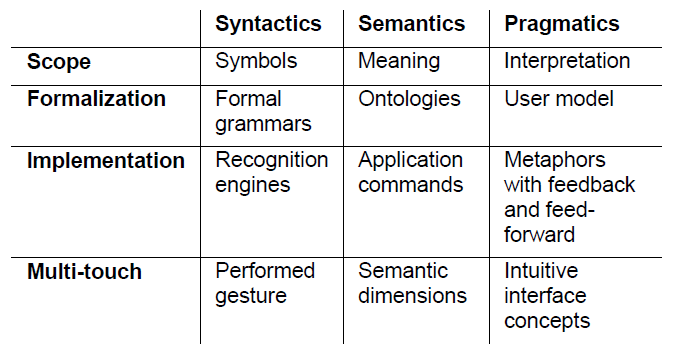
\includegraphics[scale=0.5]{Semiotics}
\end{table}
\end{comment}

% In depth understanding of the different viable gestures or signs that may be used by the user is important to formalize the syntax of gestures. The general term used for gestures is \textit{atomic gestures} \citep{kammer2010towards}. It includes basic shapes like lines, curves, and circles which may still be improved to form more complex gestures. 

% In depth understanding of the different viable gestures or signs that may be used by the user is important to formalize the syntax of gestures. Table \ref{tab:gle} shows the different language elements for GeForMT. The general term used for gestures is \textit{atomic gestures} \citep{kammer2010towards}. It includes basic shapes like lines, curves, and circles which may still be improved to form more complex gestures. 

% Other types of gestures include freeform (MOVE) in which you can assign a command for a specified gesture trail. Another is short contact (POINT, HOLD) which does not require moving the fingers (see Figure \ref{fig:atomicgestures}). One can also specify the direction of a gesture trail like in the case of LINE\_NE.

% Multi-touch also supports simultaneous contacts which can be customized as well using the \textit{composition operators} of GeForMT. Synchronous movements are identified using the asterisk symbol (*) while asynchronous movements are identified using the plus-sign (+). A sequence of atomic gestures may also be defined using a comma delimiter (,). In order to define how two or more atomic gestures relate with one another, prefixes are used. The CROSS prefix is used to indicate overlaps, SYNC for parallel movements, JOIN for converging motion, and SPREAD for separating motion.

% In depth understanding of the different viable gestures or signs that may be used by the user is important to formalize the syntax of gestures and so the research also discussed different possible gestures. Table \ref{tab:gle} shows the different language elements for GeForMT. The general term used for gestures is \textit{atomic gestures} \citep{kammer2010towards}. It includes basic shapes like lines, curves, and circles which may still be improved into more complex gestures. Other types of gesture include freeform (MOVE) in which you can assign a command for a specified gesture trail, and short contact (POINT, HOLD) which does not require movement of fingers (Figure \ref{fig:atomicgestures}). Another type is DEPOINT which refers to the lifting of finger or hands and it can be used as a part of another gesture. Different attributes may be customized depending on the desired gesture. An example would be specifying the direction of a gesture trail (e.g. LINE\_NORTH) and adding focus which is a list of objects used as identifiers. Multi-touch also supports simultaneous contacts which can be customized as well using the \textit{composition operators} of GeForMT. Synchronous movements are identified using the asterisk symbol (*) while asynchronous movements are identified using the plus-sign (+). A sequence of atomic gestures may also be defined using a comma delimiter (,). In order to define how two or more atomic gestures relate with one another, prefixes are used. The CROSS prefix is used to indicate overlaps, SYNC for parallel movements, JOIN for converging motion, and SPREAD for separating motion.

\begin{comment}
\begin{table}[H]
	\centering
    
    \caption{Language elements for GeForMT \citep{kammer2010towards}} \label{tab:gle}
	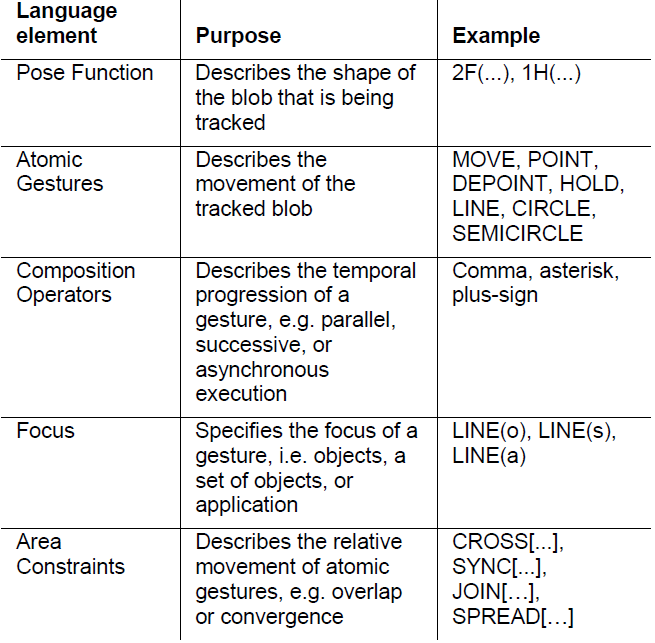
\includegraphics[scale=0.5]{GeForMTLanguageElements}
    
\end{table}

\end{comment}

\begin{figure}[H]
	\centering
	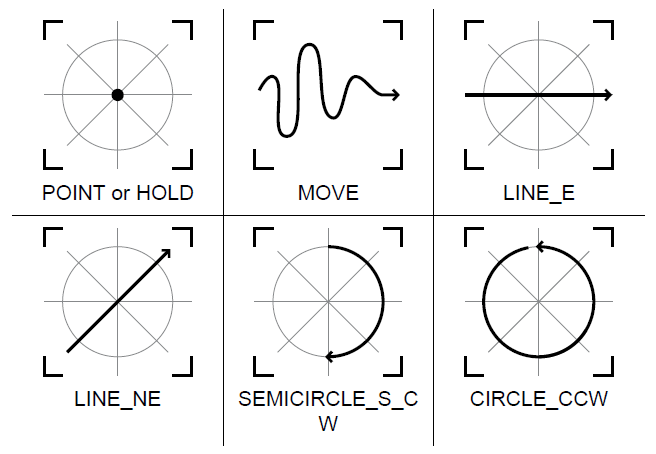
\includegraphics[scale=0.4]{AtomicGestures}
    \caption{Examples of atomic gestures \citep{kammer2010towards}.}
    \label{fig:atomicgestures}
\end{figure}

% The EyesWeb system, developed in the study of \citet{camurri2000eyesweb}, attempts to generate music through human body movement or gestures. The system is equipped with a camera that can detect movements. Its goal is to generate music that is appropriate to the movement it detects \citep{camurri2000eyesweb}. However, since it was an initial study, the system was still limited in terms of movement detection.

The same idea is found in the study of \cite{ip2005cyber}, where a system called the Cyber Composer was developed to make use of hand gestures to create music (see Figure \ref{fig:cybercomposer-media}). The system generated music from blueprints for musical structures. These can be accessed and modified through the use of an external input device called the CyberGlove. This form of input was considered helpful for people without any background in composition. With the help of the CyberGlove, they could create music with only simple hand gestures \citep{ip2005cyber}. However, despite the help provided by the CyberGlove, it was still found to be obtrusive and inaccessible. 

\begin{figure}[H]
	\centering
	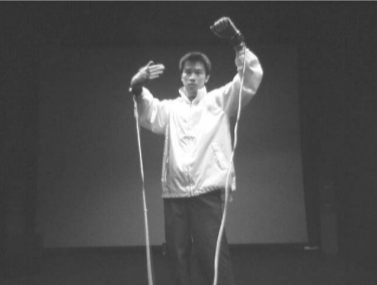
\includegraphics[scale=0.7]{cyberGloveUse}
    \caption{A user operating the CyberGlove \citep{ip2005cyber}.}
    \label{fig:cybercomposer-media}
\end{figure}

In the study of \citet{epps2006a}, the use of gesture interactions as a method of input for tabletop displays was explored. It was found that the index finger was commonly used by the testers when interacting with a large, flat display. Thus, the study recommends to build gesture interactions that mainly revolve around the use of the index finger \citep{epps2006a}.

The aforementioned study of \citet{kikuchi2016music} also used gestures through the use of the Surface Pen. The developed system's mode of interaction involved using the Surface Pen to interact with a Microsoft Surface Pro 3's touchscreen. The simplified interface and intuitive interaction was found to be helpful for inexperienced composers write music.

% The work of \citet{kazi2012vignette} illustrated a similar approach to that of \citet{kikuchi2016music}. 

\citeauthor{kazi2012vignette} developed Vignette, an interactive illustration tool that allows users to manipulate textures through the use of freeform gestures. Although not a musical composition tool, Vignette has similar goals in that it aims to provide an easy-to-use interface that incorporates gestures to augment the illustration process. Texture manipulations such as duplication, synthesis, and fillings can be easily done in Vignette through simple gestures made in the interface \citep{kazi2012vignette}. The overall impressions of users during evaluation were positive, and comments were that it was easy to learn and allowed them to create quick illustrations in only a short time of use.

The later work of \citet{kazi2014draco} builds on Vignette by extending it to allow animations. The new tool, called Draco, is a sketch and animation tool that provides a simplified interface for animation through the use of \textit{kinetic textures}, which is their developed framework for endowing sketched components with motion properties. It allows users to easily create simple animations through intuitive gestures and freeform strokes. Raindrops can be animated by drawing simple curved or linear lines that denote its direction and length of travel.

The earlier study of \citep{mo2005smartcanvas} used cameras to detect gestures. SmartCanvas is a drawing desk system that allows users to create drawings through gestures. This is done with 2 cameras that detect the type of gesture and identify whether or not the user is touching the surface. This resulted in a minimal drawing system without the need for a touchscreen \citep{mo2005smartcanvas}. However, there was one main drawback. Since users would draw on a surface and the drawing would be generated on the computer screen, the user would have to keep switching his/her focus when drawing.

\begin{landscape} % Landscape page
\begin{table} [!htbp]  
\label{tab:rsogi}        
        \captionof{table}{Related Studies on Gesture Interactions}
   \vspace{0.20cm}    
        \begin{tabular}{|p{3cm}|p{4cm}|p{4cm}| p{4cm}| p{5cm} | } %{|l|l|l}
        \hline 
       Authors & Name of Tool & Input/Modality & Types of Gestures & Comments and other findings \\ \hline
       
       \citet{kammer2010towards} & GeForMT & Multi-touch gestures & \makecell[tl]{Tap \\ Point or Hold \\ Linear gestures\\ Circular gestures} & Formalized an approach to create gestures \\ \hline
       
       % \citet{camurri2000eyesweb} & EyesWeb & Cameras & Body movement & Attempts to connect motion to music, but is still limited \\ \hline
       
       \citet{ip2005cyber} & Cyber Composer & CyberGlove & \makecell[tl]{Hand motions \\ Finger bends \\ Finger flexions} & Obtrusive, but allowed composition through hand gestures \\ \hline
       
       \citet{kikuchi2016music} & Music Composition with Recommendation & Microsoft Surface Pro 3 and Surface Pen & Tap gestures & The interface was found to be helpful for inexperienced composers \\ \hline
       
       \citet{epps2006a} & NA & Hand Gestures and Cameras & \makecell[tl]{Single-touch gestures \\ Hand-shape gestures} & The index finger was commonly used for interactions \\ \hline
       
       \citet{kazi2012vignette,kazi2014draco} & Vignette; Draco & Touchscreen device and stylus & \makecell[tl]{Freeform sketches \\ Straight lines \\ Curved lines} & The interface was easy-to-use for beginners and the gestures were intuitive \\ \hline
       
       \citet{mo2005smartcanvas} & SmartCanvas & Touch Gestures and Cameras & Freeform gestures & It was minimal but increased cognitive load due to users having to switch focus when drawing \\ \hline 
       
        \end{tabular}
\end{table}
\end{landscape}

\newpage















